
\documentclass[a0,portrait]{a0poster}

\usepackage{times,colordvi,amsmath,epsfig,float,color,multicol}

\pagestyle{empty}
\setlength{\parindent}{0cm}
\setlength{\parskip}{2ex}
\setlength{\columnsep}{3cm}
\addtolength{\textwidth}{2cm}
\addtolength{\oddsidemargin}{-1.5cm}

\renewcommand{\normalsize}{\Large}
\def\regularsize{\@setfontsize\normalsize{34pt}{37}}

\renewcommand\refname{}
\setlength{\fboxrule}{0.1cm}


% ----------------------------------------------------------------


% PMS287 CMYK=[100% 69% 0% 11.5%] RGB=[38/256 67/256 151/256]
\definecolor{qmuldarkblue}{rgb}{0.,0.1797,0.3281}

\definecolor{backgrey}{rgb}{0.93,0.93,0.93}
\definecolor{backblue}{rgb}{0.93,0.93,1}
\definecolor{backyellow}{rgb}{1,1,0.88} 

\definecolor{backred}{rgb}{1,0.9,0.9} 
\definecolor{backgreen}{rgb}{0.9,1,0.9}
\definecolor{backpink}{rgb}{1,0.9,1} 
\definecolor{backturquoise}{rgb}{0.9,1,1} 


% ----------------------------------------------------------------


\makeatletter
\renewcommand{\section}{\@startsection
        {section}                          % the name 
        {1}                                % the level
        {0mm}                              % the indent
        {-0.7\baselineskip}                % the beforeskip
        {5mm}                              % the afterskip
        {\center\Huge\color{qmuldarkblue}\bfseries}} % the style
\makeatother

\newcommand{\norm}[1]{\lVert#1\rVert}
\renewcommand{\vec}[1]{{\mbox{\boldmath$#1$}}}
\newcommand{\mat}[1]{{\mbox{\boldmath$#1$}}}
\newcommand{\reals}{{\mathbb R}}
\newcommand{\strng}[1]{{\mbox{\tt #1}}}
\newcommand{\inner}[2]{\big<\vec{#1}\cdot\vec{#2}\big>}

\def\argmax{\mathop{\rm argmax}}
\def\argmin{\mathop{\rm argmin}}

\begin{document}

\vspace{1cm}

\begin{center}
\colorbox{qmuldarkblue}
{
 \color{white}

 \parbox{1.0\textwidth}
 {
  \parbox{0.24\textwidth}
  {
   \begin{center}
   
\epsfig{file=images/logos/qmulblue.eps,width=12cm}\\[1ex]
   \end{center}
  }
  \parbox{0.5\textwidth}
  {
   \vspace{1cm}
   \begin{center}
   \textrm
   {
    {\veryHuge \bf \em Ordinal Regression in Evolutionary Computation}\\[1ex]
    {\huge       Thomas Philip Runarsson}
   }    
   \end{center}
   \vspace{1cm}
  }
  \parbox{0.24\textwidth}
  {
   \begin{center}
    {\huge Science Institute\\University of Iceland}\\[1ex]
   \textrm
   {
    \Large
    tpr@hi.is\\
    http://www.hi.is/\ \~\ tpr\\
   }
   \end{center}
  }
 }
}
\end{center}

\vspace{1cm}


% ----------------------------------------------------------------


\begin{multicols}{2}

\fcolorbox{black}{white}{\parbox{1.0\columnwidth}
{
\section{Introduction}

\begin{itemize}
\item The aim is to reduce the number of costly fitness
  evaluations needed in evolutionary computing.
\item The fitness of individual points is indirectly estimated
  by modeling their rank using \emph{ordinal regression or kernel
  based preference learning}.
\item A generic framework for surrogate ranking using ordinal
regression in evolutionary computation is presented. 
\item The formulation does not need an explicitly defined
  fitness function, making it suitable for {\bf co-evolution} and
  {\bf interactive evolution}.
\end{itemize}

\ \\}}

\vspace{1cm}
\fcolorbox{black}{backgrey}{\parbox{1.0\columnwidth}
{
\section{Ordinal Regression}

The ranking problem is specified by a set $S =
\{(\vec{x}_i,y_i)\}_{i=1}^\ell \subset X \times Y$ of point/rank
pairs, where $Y=\{r_1,\ldots,r_\ell\}$ is the outcome space with
ordered ranks $r_1> r_2,> \ldots > r_\ell$.

\ \\ 
In ordinal regression the task is to obtain a function  that
can for a given pair $(\vec{x}_i,y_i)$ and $(\vec{x}_j,y_j)$
distinguish between two different outcomes: $y_i > y_j$ and $y_j
> y_i$.

\ \\
The training set is as follows:
$$S' = \big\{(\vec{x}_k^{(1)},
\vec{x}_k^{(2)}),t_k=\text{sign}(y_k^{(1)} -
y_k^{(2)})\big\}_{k=1}^{\ell'}$$
where $(y_k^{(1)} = r_i) \wedge
(y_k^{(2)} = r_{i+1})$ (and vice versa $(y_k^{(1)} = r_{i+1})
\wedge (y_k^{(2)} = r_{i})$) resulting in $\ell'=2(\ell-1)$
possible adjacently ranked training pairs. The rank difference
is denoted by $t_k\in[-1,1]$.

\ \\
A Support Vector Machine (SVM) is used on the above training
data.

\ \\}}

\vspace{1cm}
\fcolorbox{black}{backblue}{\parbox{1.0\columnwidth}
{
\section{Model Selection}

Two kernel types  are investigated, the
\emph{polynomial kernel}
\begin{equation}
\kappa(\vec{x}_i,\vec{x}_j) = (1 + \inner{x_i}{x_j})^d
\end{equation}
and \emph{Gaussian kernel}
\begin{equation}
\kappa(\vec{x}_i,\vec{x}_j) = \exp\big(-\gamma \norm{\vec{x}_i-\vec{x}_j}^2\big).
\end{equation}

\ \\
When applying kernel methods it is important to scale the
points $\vec{x}$ first. A standard method of doing so is to
scale the training set such that all points are in some range,
typically $[-1,1]$. That is, scaled $\tilde{\vec{x}}$ is
\begin{equation}
\tilde x_i = 2 (x_i - \underline{x}_i) / (\overline{x}_i -
\underline{x}_i) - 1 ~~~ i = 1,\ldots,n
\end{equation}
where $\underline{x}_i$, $\overline{x}_i$ are the maximum and
minimum values of variable $i$ in set $S$.

\vspace{0.8cm}}}

\vspace{1cm}
\fcolorbox{black}{backblue}{\parbox{1.0\columnwidth}
{
\section{Model Improvement}

\begin{enumerate}
\item Estimate the ranking of a population of points of unknown
  fitness using the current surrogate. Let the point with the
  highest ranking be a test point, $\vec{x}_t$. Rank this test
  point with respect to the points in the training set using the
  current surrogate.
\item Evaluate the test point using the true fitness function
  and evaluate its true rank among the training points.
\item Compare the rankings by computing the rank
  correlation $\tau_k$ (Kendall's $\tau$) for the ranking in 1 and 2.
\item Add this new point to the training set.
\item If $\tau_k$ is equal to $1$ the model is said to be
  sufficiently accurate. This is a simple cross-validation
on a single test point.
\item If $\tau_k < 1$ the model is not sufficiently accurate. In
  this case update the surrogate using the new training set.
  Repeated the steps above until $\tau=1$ or all points of
  unknown fitness have been evaluated.
\end{enumerate}
\vspace{0.8cm}}}

\vspace{1cm}
\fcolorbox{black}{white}{\parbox{1.0\columnwidth}
{
\section{Experimental Studies}

\begin{itemize}
\item Method tested using the CMA-ES on a few test functions.
\item Illustrative example for different training size and
  kernel types for Rosenbrock's function:
\end{itemize}

\begin{center}
\begin{tabular}{c@{ }c@{ }c}
\resizebox*{0.33\columnwidth}{!}{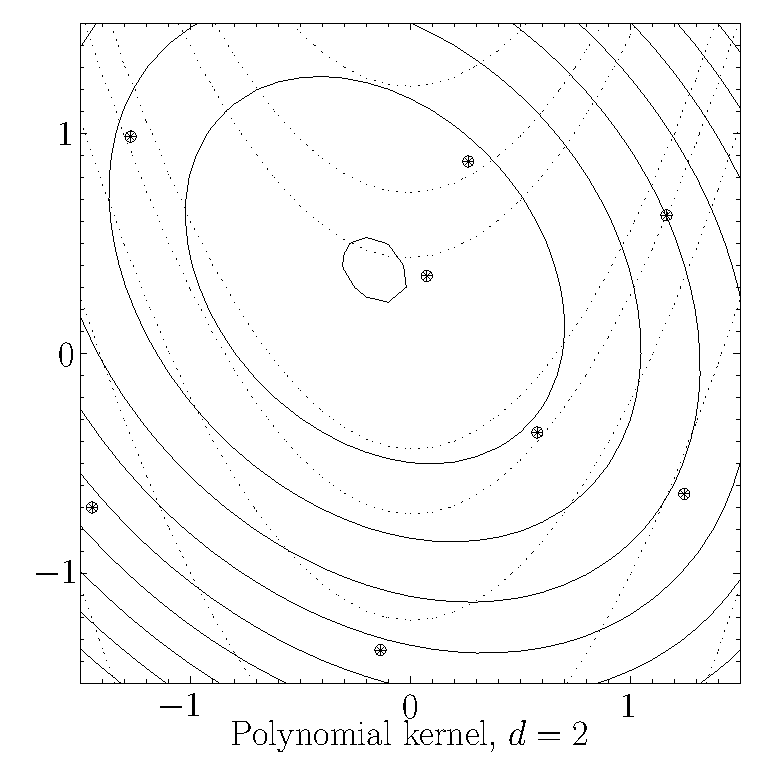
\includegraphics[height=0.33\columnwidth]{figs/poly2global10.eps}} &
\resizebox*{0.305\columnwidth}{!}{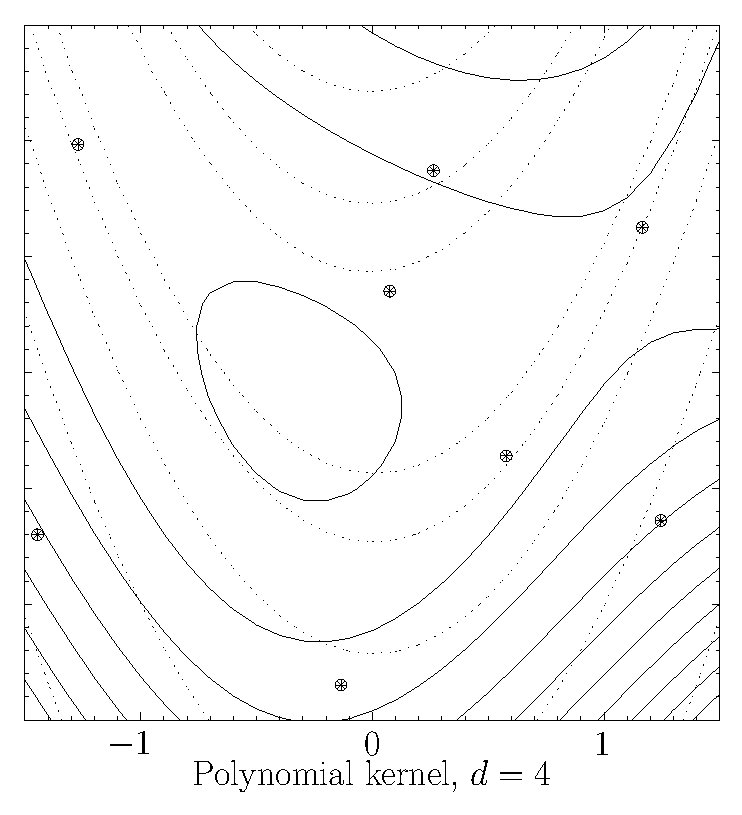
\includegraphics[height=0.33\columnwidth]{figs/poly4global10.eps}} &
\resizebox*{0.305\columnwidth}{!}{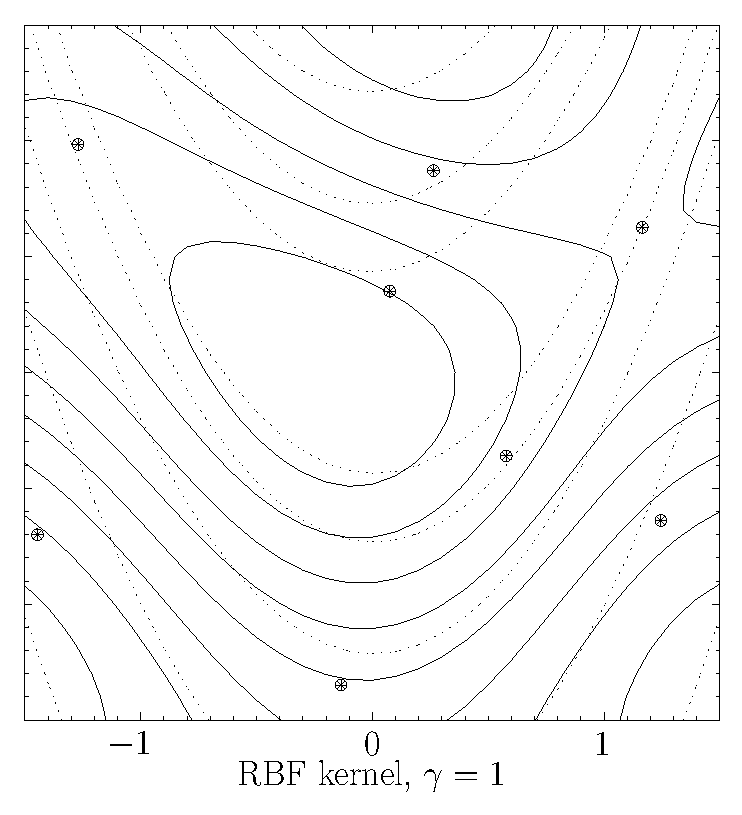
\includegraphics[height=0.33\columnwidth]{figs/rbf1global10.eps}} \\
\resizebox*{0.33\columnwidth}{!}{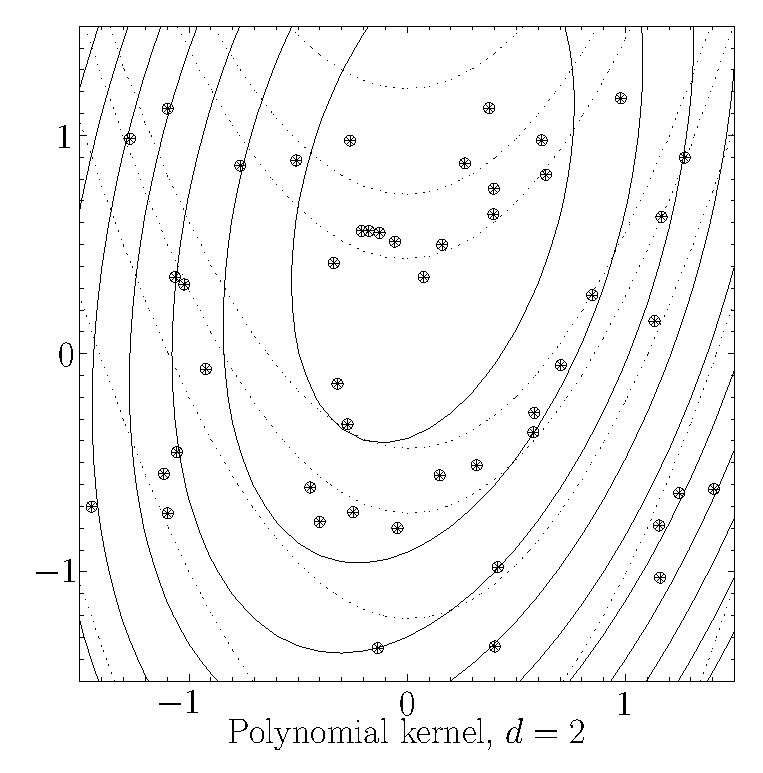
\includegraphics[height=0.33\columnwidth]{figs/poly2global.eps}} &
\resizebox*{0.305\columnwidth}{!}{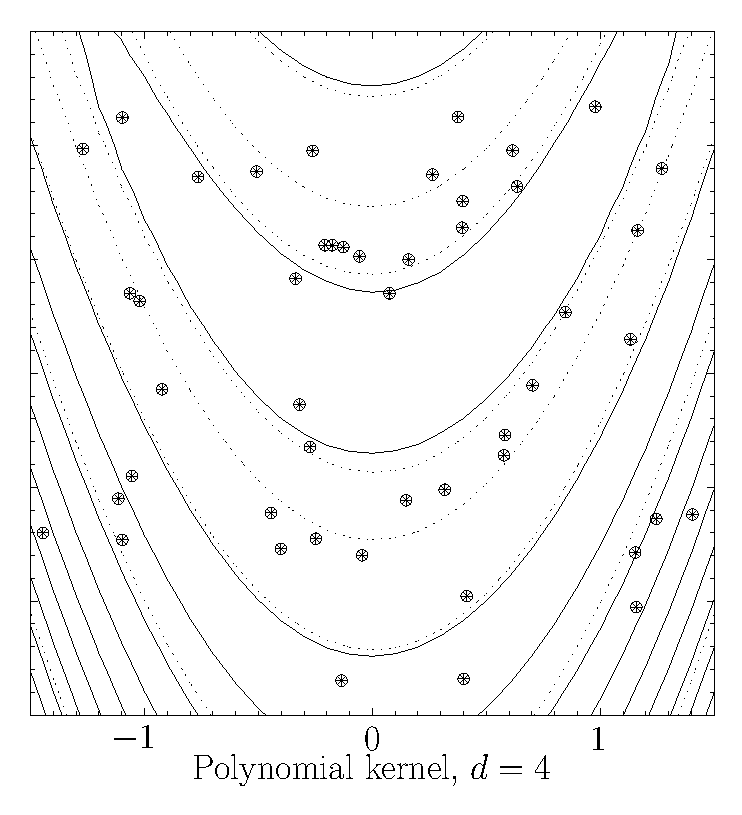
\includegraphics[height=0.33\columnwidth]{figs/poly4global.eps}} &
\resizebox*{0.305\columnwidth}{!}{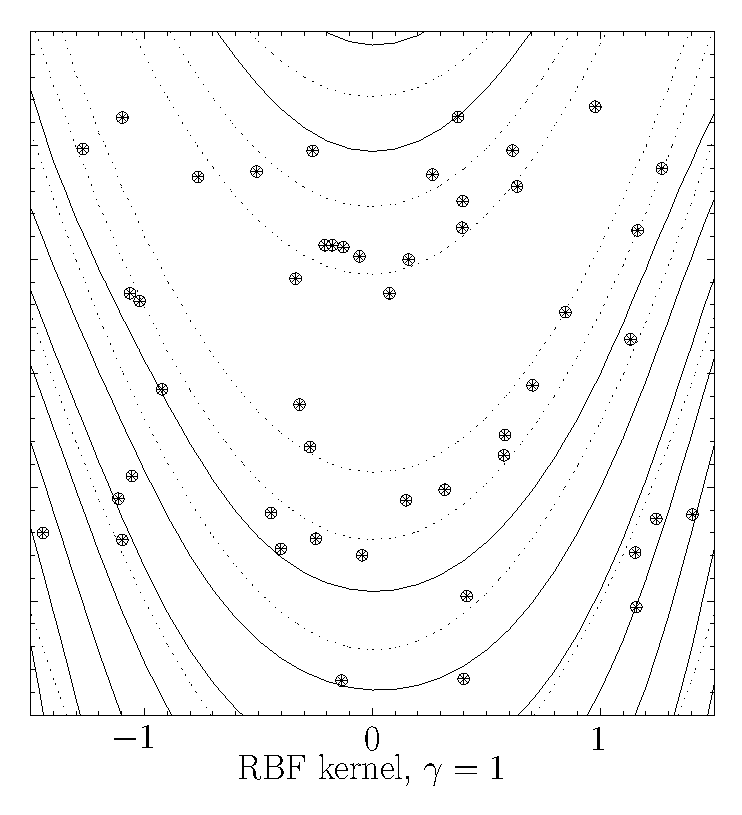
\includegraphics[height=0.33\columnwidth]{figs/rbf1global.eps}} \\
\end{tabular}
\end{center}
}}

\vspace{1cm}
\fcolorbox{black}{backyellow}{\parbox{1.0\columnwidth}
{
\section{Conclusions}

\begin{itemize}
\item First time surrogate ranking is used in evolutionary computing.
\item Reduces the number of fitness evaluations needed
  during evolution.
\item Can be applied to more abstract data types as long as a
  kernel can be defined, for example a tree kernel for GP.
\item May be sensitive to the model selected and training set size.
\item Currently the author is applying the technique to Pareto
  ranking for multi-objective optimization.
\end{itemize}
}}

\end{multicols}


% ----------------------------------------------------------------


%\vspace{-1cm}
%\small
\begin{thebibliography}{10}

\bibitem{Kender98}
J.R. Kender and B.L. Yeo.
\newblock Video scene segmentation via continuous video coherence.
\newblock In {\em {IEEE} Conference on Computer Vision and Pattern
  Recognition}, pages 367--373, Santa Barbara, June 1998.

\bibitem{Graves02}
A.P. Graves and M.~Lalmas.
\newblock Video retrieval using an {MPEG-7} based inference network.
\newblock In {\em International {ACM SIGIR} Conference on Research and
  Development in Information Retrieval}, pages 339--346, Tampere, Finland,
  August 2002.

\bibitem{Xiang02}
T.~Xiang, S.~Gong, and D.~Parkinson.
\newblock Autonomous visual events detection and classification without
  explicit object-centred segmentation and tracking.
\newblock In {\em Proc of British Machine Vision Conference}, volume~1,
  pages 233--242, Cardiff, September 2002.

\end{thebibliography}
\normalsize

\vspace{0.5cm}

\colorbox{qmuldarkblue}
{
 \color{white}
 \parbox{1.0\textwidth}
 {
  \vspace{0.2cm}

  \begin{center}
  Parallel Problem Solving from Nature PPSN - IX.
  \end{center}

  \vspace{0.2cm}
 }
}


\end{document}
